\documentclass[paperwidth=30in,paperheight=40in,fontscale=0.35]{baposter} % Adjust the font scale/size here

\usepackage{graphicx} % Required for including images
\graphicspath{{figures/}} % Directory in which figures are stored
\usepackage{microtype} % Super-detailed letter spacing (and less box warnings from LateX)
\usepackage{palatino}
\usepackage[font=small, labelfont=bf]{caption} % Required for captions
\setlength{\abovecaptionskip}{0pt}  % Reduce spacing above and below captions
\setlength{\belowcaptionskip}{0pt}
\usepackage{tcolorbox} % Allows us to make the colored boxes for the headers
\usepackage[style=nature, isbn=false, doi=false, url=false]{biblatex} % Use biblatex to manage references
\bibliography{spiral} % Point to the bibliography file
\definecolor{reallylightgray}{gray}{0.88} % defining a color to use

\newtcolorbox{coloredbox}[1]{% New command to make a colored header box
  colback=SkyBlue,
  colframe=SkyBlue,
  rounded corners,
  center,
  height=15mm,
  width=#1
}

\hbadness=1800  % Stop complaining about overfull references

\begin{document}
\begin{poster}
{% Options
headerborder=open, % Adds a border around the header of content boxes
colspacing=5mm, % Column spacing
bgColorOne=white, % Background color for the gradient on the left side of the poster
bgColorTwo=white, % Background color for the gradient on the right side of the poster
borderColor=black, % Border color
headerColorOne=reallylightgray, % Background color for the header in the content boxes (left side)
headerColorTwo=reallylightgray, % Background color for the header in the content boxes (right side)
headerFontColor=black, % Text color for the header text in the content boxes
boxColorOne=reallylightgray, % Background color of the content boxes
textborder=roundedsmall, % Format of the border around content boxes, can be: none, bars, coils, triangles, rectangle, rounded, roundedsmall, roundedright or faded
eyecatcher=true, % Set to false for ignoring the left logo in the title and move the title left
headerheight=0.095\textheight, % Height of the header
headershape=smallrounded, % Specify the rounded corner in the content box headers, can be: rectangle, small-rounded, roundedright, roundedleft or rounded
headerfont=\Large\bf\textsc, % Large, bold and sans serif font in the headers of content boxes
%textfont={\setlength{\parindent}{1.5em}}, % Uncomment for paragraph indentation
linewidth=0pt, % Width of the border lines around content boxes
}
{} % First university/lab logo on the left
{\textbf{Self-improvement through Bayesian optimization:\\A conceptual experiment}\vspace{2mm}} % Poster title
{% Authors
    \textsc{Kevin Tran | Art and Machine Learning | Spring 2019} \\
}
{
\includegraphics[height=0.07\textheight]{CMU_Logo_Stack_Red.eps}} % Second university/lab logo on the right


%%%%%%%%%%%%%%%%%%%%%%%%%%%%%%%%%%%%%%%%%%%%%%%%%%%%%%%%%%%%
% References
%%%%%%%%%%%%%%%%%%%%%%%%%%%%%%%%%%%%%%%%%%%%%%%%%%%%%%%%%%%%
\headerbox{References}{name=references, column=2, above=bottom}{% Make the header
\small{% Reduce the font size in this block
    \printbibliography[heading=none]{}
    }}


%%%%%%%%%%%%%%%%%%%%%%%%%%%%%%%%%%%%%%%%%%%%%%%%%%%%%%%%%%%%
% Concept
%%%%%%%%%%%%%%%%%%%%%%%%%%%%%%%%%%%%%%%%%%%%%%%%%%%%%%%%%%%%
\headerbox{% Create the header
    \begin{coloredbox}{34mm}
        Concept
    \end{coloredbox}
    }{name=concept, column=0, row=0}{% Location of this box

A person's journey through life and their subsequent growth is a compelling topic that is
used archetypically throughout humanity's history of story-telling and art. The idea that
we can rise above adversity and become better than who we are is fascinating to us. I
wanted to experiment with this idea of continuous self-improvement. I focus especially on
the journey of personal growth rather than the final result.

This concept is what led me to develop an algorithm that evokes this journey of
continuous self-improvement. Here I use a combination of emotion classifiers and Bayesian
optimization to turn human portraits into abstract ``avatars'' of various virtues, and I
use this algorithm to show that even the worst version of us can better ourselves and
still rise above iniquity.
}


%%%%%%%%%%%%%%%%%%%%%%%%%%%%%%%%%%%%%%%%%%%%%%%%%%%%%%%%%%%%
% Background
%%%%%%%%%%%%%%%%%%%%%%%%%%%%%%%%%%%%%%%%%%%%%%%%%%%%%%%%%%%%
\headerbox{% Create the header
    \begin{coloredbox}{47mm}
        Background
    \end{coloredbox}
    }{name=background, column=0, below=concept, above=bottom}{% Location of this box

    I wanted an algorithm that starts with a human portrait as an input and then modifies
    it iteratively. Style transfer\textsuperscript{\cite{Gatys2015}}
    (Figure~\ref{fig:style_xfer}) is well suited for image modification. Style transfer
    superimposes the style of one image onto a content image without changing the
    high-level features of the content image.

    \begin{center}
        \vspace{-5mm}
        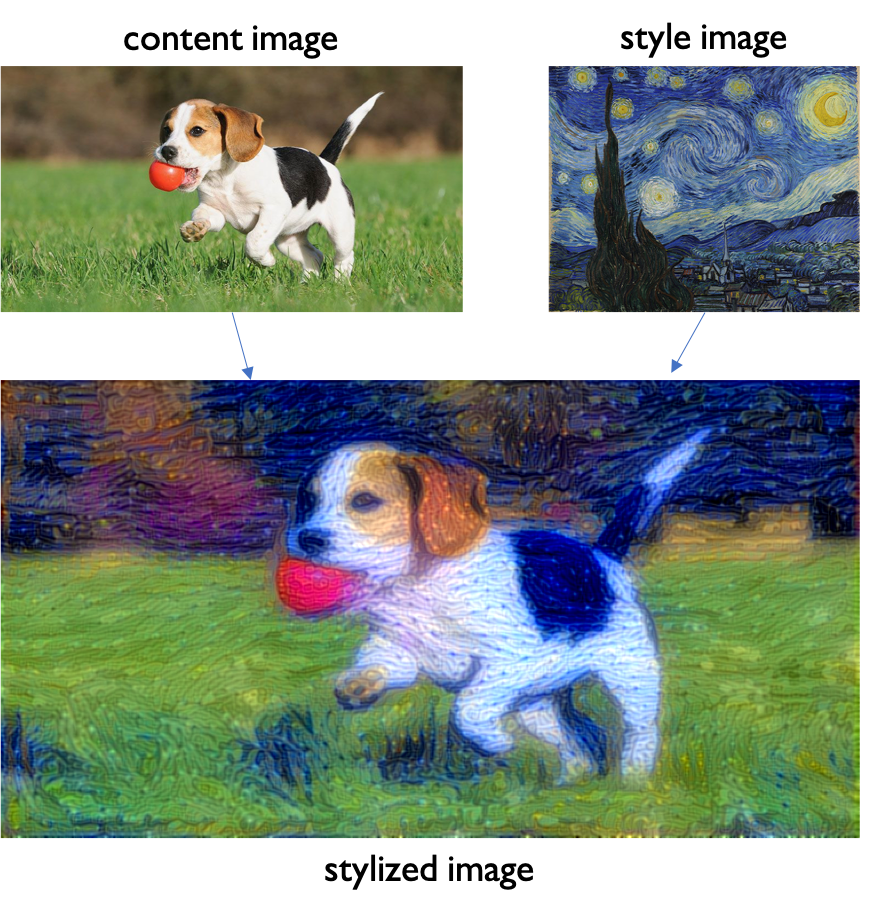
\includegraphics[width=\linewidth]{style_transfer}
        \captionof{figure}{The style of ``Starry Night'' transferred onto an image of a
        puppy to make a ``Starry Puppy''. This method was used to modify human portraits
        given various style images.}\label{fig:style_xfer}
    \end{center}

    But how do we know whether we are changing the images for better or for worse?
    Various convolutional neural networks exist for classifying the sentiment and/or
    emotion of an image,\textsuperscript{\cite{Jou2016, Alvarez-Melis2017}} but most seem
    closed source. Thankfully there are public datasets of images labeled with ther
    associated emotions,\textsuperscript{\cite{Mohammad2018}} which can be used to train
    our own ``virtue/iniquity'' classifiers.

    We also need an iterative method for choosing which style images to use at each point
    in time. Bayesian optimization is well suited for this task (Figure~\ref{fig:bo}).
    Many packages exist to perform Bayesian optimization, such as CMU's
    Dragonfly.\textsuperscript{\cite{Kandasamy2019}}

    \begin{center}
        \includegraphics[width=\linewidth]{BO}
        \captionof{figure}{Bayesian optimization is the process of using a Gaussian
        process regressor to optimize some expensive, black-box objective function. In
        this case, we will be optimizing an image to fit a virtue. Figure taken from
        Kandasamy et al.\textsuperscript{\cite{Kandasamy2019}}}\label{fig:bo}
    \end{center}
} % chktex 10


%%%%%%%%%%%%%%%%%%%%%%%%%%%%%%%%%%%%%%%%%%%%%%%%%%%%%%%%%%%%
% Method
%%%%%%%%%%%%%%%%%%%%%%%%%%%%%%%%%%%%%%%%%%%%%%%%%%%%%%%%%%%%
\headerbox{% Create the header
    \begin{coloredbox}{34mm}
        Method
    \end{coloredbox}
    }{name=method, column=1, row=0}{% Location of this box

    \begin{center}
        \vspace{-2mm}
        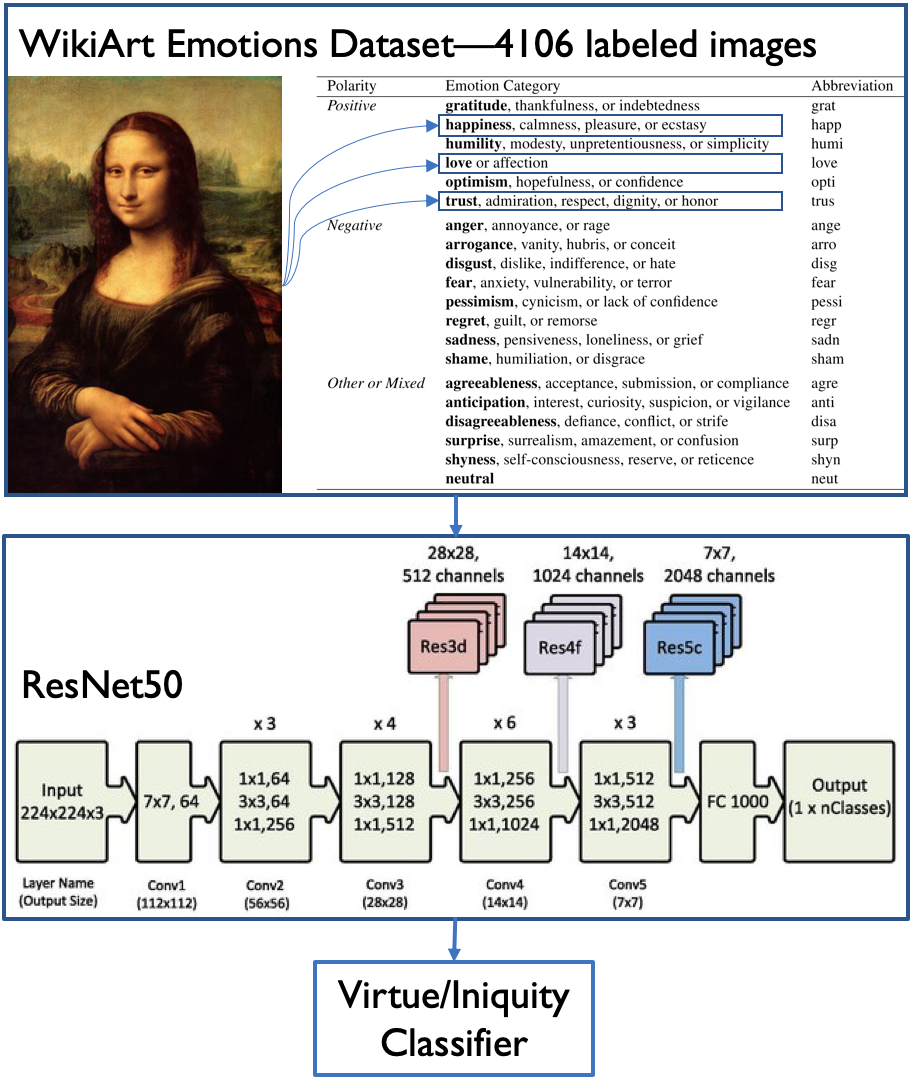
\includegraphics[width=\linewidth]{vic}
        \captionof{figure}{We use the WikiArt Emotions
        dataset\textsuperscript{\cite{Mohammad2018}} to train
        ResNet50\textsuperscript{\cite{He2015}}, creating a neural network that can
        classify an image's virtue/iniquity.}\label{fig:vic}
    \end{center}

    I first trained a classifier (Figure~\ref{fig:vic}) that can quantify an image's
    associated virtue/iniquity. I then incorporated the classfier within a Bayesian
    optimization framework to choose new images to perform style transfer with
    (Figure~\ref{fig:spiral_out}).

    \begin{center}
        \vspace{-2mm}
        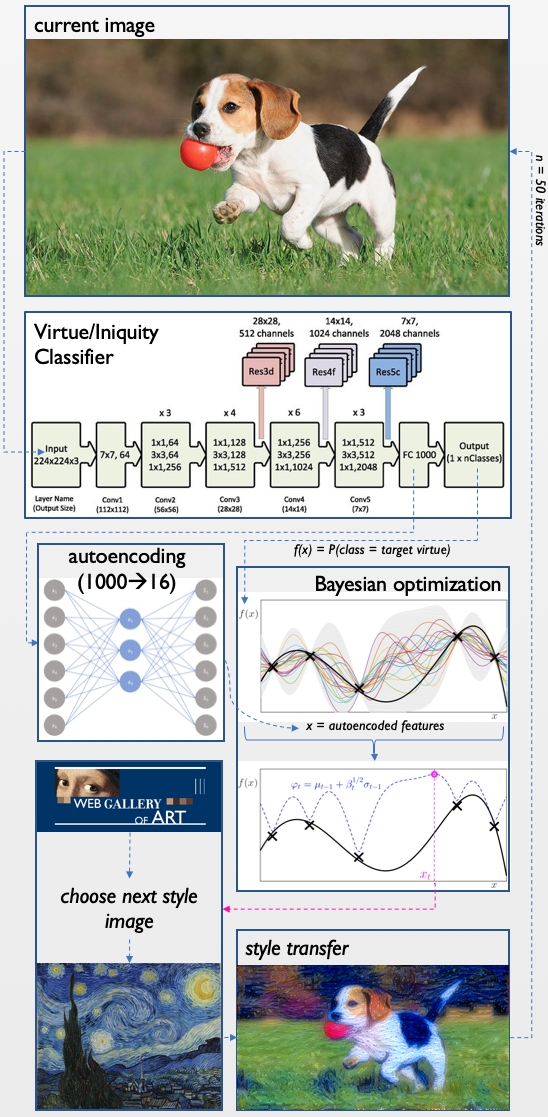
\includegraphics[width=\linewidth]{spiral_out}
        \captionof{figure}{My algorithm for iterative style transfer. The goal is to
        modify an image such that it begins to match the target virtue more and more
        closely.}\label{fig:spiral_out}
    \end{center}
} % chktex 10


%%%%%%%%%%%%%%%%%%%%%%%%%%%%%%%%%%%%%%%%%%%%%%%%%%%%%%%%%%%%
% Results
%%%%%%%%%%%%%%%%%%%%%%%%%%%%%%%%%%%%%%%%%%%%%%%%%%%%%%%%%%%%
\headerbox{% Create the header
    \begin{coloredbox}{32mm}
        Results
    \end{coloredbox}
    }{name=results, column=2}{% Location of the box

    \begin{center}
        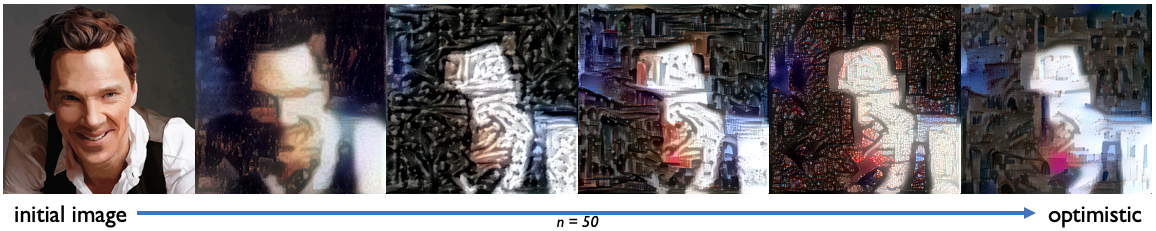
\includegraphics[width=\linewidth]{cumberbatch}
        \captionof{figure}{Turning Cumberbatch optimistic.}\label{fig:cumberbatch}
        \vspace{-2mm}
    \end{center}

    Figure~\ref{fig:cumberbatch} shows how the algorithm transforms a portrait using the
    ``optimistic'' virtue. As a conceptual experiment, I turned Gaius Baltar into both
    an avatar of both arrogance and humility. I then tried to see if I could transform an
    arrogant Baltar into a humble one (Figure~\ref{fig:baltar}).

    \begin{center}
        \vspace{-3mm}
        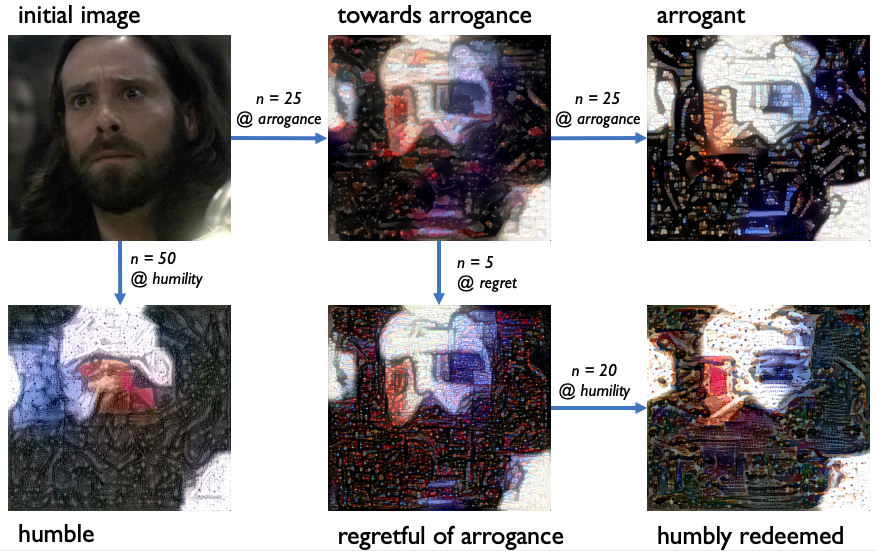
\includegraphics[width=\linewidth]{baltar}
        \captionof{figure}{Possible paths of Gaius Baltar's character
        progression.}\label{fig:baltar}
    \end{center}
}


%%%%%%%%%%%%%%%%%%%%%%%%%%%%%%%%%%%%%%%%%%%%%%%%%%%%%%%%%%%%
% Future Work
%%%%%%%%%%%%%%%%%%%%%%%%%%%%%%%%%%%%%%%%%%%%%%%%%%%%%%%%%%%%
\headerbox{% Create the header
    \begin{coloredbox}{47mm}
        Future Work
    \end{coloredbox}
    }{name=future, column=2, below=results, above=references}{% Location of the box

    The final result seems to be more dependent on the total number of iterations rather
    than the target attributes. This could be addressed by using a better set of
    candidate style images---e.g., instead of using The Web Gallery of Art, images
    created by an emotional GAN\textsuperscript{\cite{Alvarez-Melis2017}}
    (Figure~\ref{fig:egan}) might be more effective.

    \begin{center}
        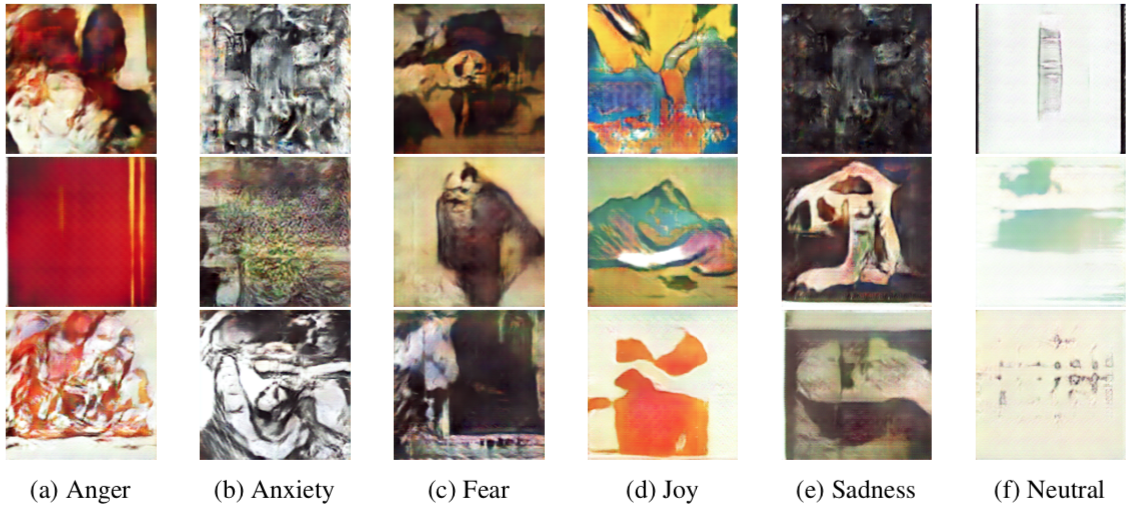
\includegraphics[width=\linewidth]{eGAN}
        \captionof{figure}{Example images created by a
        GAN\textsuperscript{\cite{Alvarez-Melis2017}} that can create images that evoke
        particular emotions.}\label{fig:egan}
    \end{center}
}


\end{poster}
\end{document} % chktex 17
